\section*{31. Основное уравнение магнитостатики и его общее решение для
безграничного пространства. Магнитный диполь. Вектор-потенциал и
магнитное поле диполя.}
 
\subsection*{Основное уравнение магнитостатики и его общее решение для
безграничного пространства}

Воспользуемся уравнением магнитостатики:

\[
\mathrm{rot}\vec{H}=\frac{4\pi}{c}\vec{j}  
\]

и подставим его в:

\[
\vec{H}=\mathrm{rot}\vec{A}
\]

Получим:
\[
\mathrm{rot}(\mathrm{rot}\vec{A} )=\frac{4\pi}{c}\vec{j}  
\]

Двойной ротор в левой части уравнения преобразуем, используя известную формулу векторного анализа:

\[
\mathrm{rot}(\mathrm{rot}\vec{A} )=-\Delta \vec{A}+ \grad \mathrm{div}\vec{A} 
\]

и используем кулоновскую калибровку потенциала:

\[
\mathrm{div}\vec{A}=0 
\]

В результате получим \textit {основное уравнение} магнитостатики:

\[
\boxed{\Delta \vec{A}=-\frac{4\pi}{c}\vec{j} }
\]

По аналогии с уравнением Пуассона $\Delta\varphi=-4\pi\rho$ и его общим решением $\varphi(\vec{r})=\int \frac{\rho(\vec{r'}dV')}{|\vec{r}-\vec{r'}|}=\frac{q}{|\vec{r}-\vec{r'}|}$ нетрудно догадаться, что общее решение уравнения можно записать следующим образом:

\[
\boxed{\vec{A}=\frac{1}{c}\int \frac{\vec{j}(\vec{r'})dV'}{|\vec{r}-\vec{r'}|}  }
\]

\subsection*{Магнитный диполь и Вектор-потенциал и
Магнитное поле диполя}

\begin{center}
    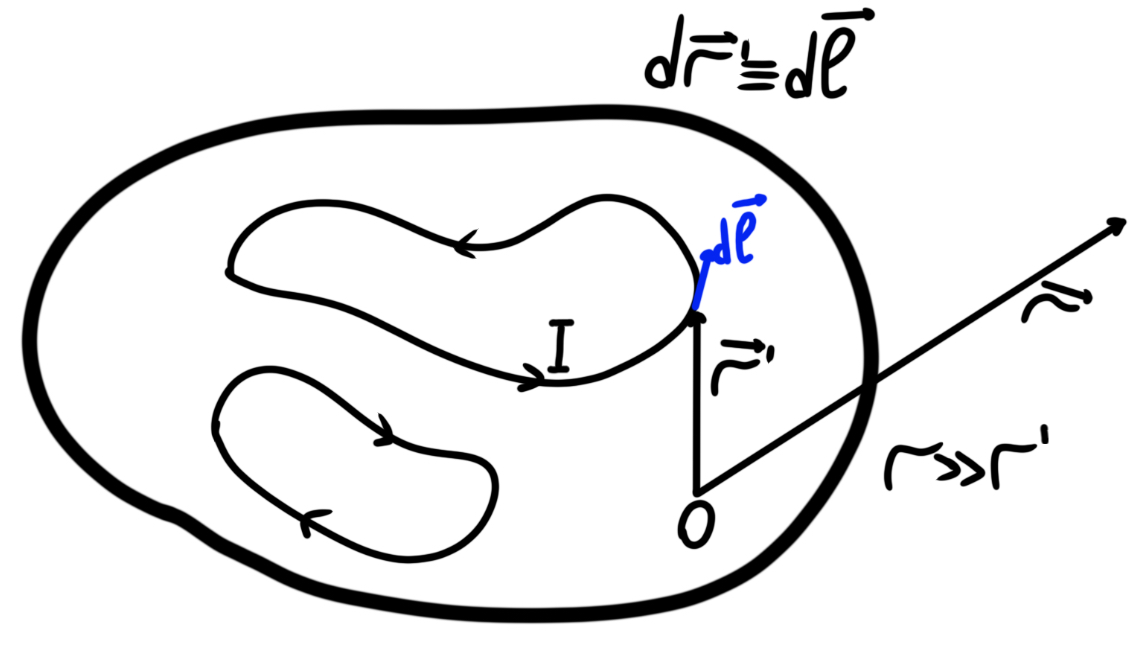
\includegraphics[width=0.5\textwidth]{im/69.png}
\end{center}

\begin{gather*}
    \vec{A}=\frac{q}{c} \iiint \frac{\vec{j}(\vec{r'})}{|\vec{r}-\vec{r'}|}dV'=\sum \frac{I}{c}\oint \frac{1}{|\vec{r}-\vec{r'}|}d\vec{r'} \\
    \text{в дальнейших формулах не будем писать }\Sigma \\
    \vec{j}dV'\rightarrow Id\vec{l}=Id\vec{r'} 
\end{gather*}

Вспомним разложение:

\[
\frac{1}{|\vec{r}-\vec{r'}|} =\frac{1}{r}+\frac{\vec{r}\cdot\vec{r'}}{r^3}+\dots (\text{ограничемся двумя членами})
\]

\begin{gather*}
    \vec{A}
\end{gather*}